\documentclass[11pt]{article}
\usepackage[utf8]{inputenc}
\usepackage[T1]{fontenc}
\usepackage{lmodern}
\usepackage{amsmath, amssymb}
\usepackage{graphicx}
\usepackage{booktabs}
\usepackage[margin=2.4cm]{geometry}
\usepackage[french]{babel}
\usepackage{caption}
\captionsetup{font=small, labelfont=bf}

\title{Satellites d'observation de la Terre}
\author{Etienne Chevrolat}
\date{}

\begin{document}

\maketitle

\begin{abstract}
\noindent Ce rapport dresse un panorama chiffré de la population des satellites d'observation de la Terre : combien ils sont, à qui ils appartiennent, sur quelles orbites ils volent et pourquoi, à quoi servent leurs missions, et comment ils manœuvrent.
\end{abstract}

\section*{Points clés}

\begin{center}
\fbox{\begin{minipage}{0.93\textwidth}
\vspace{2pt}
\begin{itemize}\setlength{\itemsep}{2pt}
  \item \textbf{$\sim$1\,200 satellites} d'observation de la Terre actifs fin 2022, soit \textbf{17\,\%} des satellites actifs à cette date = deuxième usage après les télécommunications.
  \item \textbf{95\,\%} d'entre eux sont en orbite LEO, et l'essentiel dans une bande d'inclinaison très étroite autour de $98^\circ$.
  \item \textbf{Les 10 premiers opérateurs détiennent la moitié du parc}, et les trois premiers sont des opérateurs de constellations (Planet, Spire, ministère de la Défense chinois).
  \item \textbf{États-Unis et Chine} pèsent à eux seuls environ 44\,\% du parc rien que par leurs opérateurs du top 10.
  \item \textbf{1960} : premières images depuis l'espace, météo civile et reconnaissance militaire la même année. \textbf{1972} : ouverture civile avec Landsat-1. \textbf{1986} : première vente commerciale d'images avec SPOT-1.
  \item \textbf{$\sim$5\,700 satellites d'observation} sont attendus au lancement sur 2025--2034, soit près du triple de la décennie écoulée.
\end{itemize}
\vspace{2pt}
\end{minipage}}
\end{center}

\section{Définition}

On qualifie de satellite d'observation de la Terre toute charge utile dont la mission principale est l'analyse et détection de la surface, de l'océan ou de l'atmosphère terrestres. Cela exclut les télécommunications, la navigation et les relais de données, mais inclut la météorologie et l'altimétrie.

Jusqu'aux années 2010, cette population était dominée par une centaine de plateformes institutionnelles lourdes. Elle est aujourd'hui portée, en nombre, par des constellations commerciales de petits satellites. Cette bascule est le fait structurant du domaine : ça change qui possède les satellites, sur quelles orbites ils volent, et comment ils manœuvrent.

\section{Combien de tels satellites}

La dernière photographie complète et publique du parc est 
la base de l'Union of Concerned Scientists, en décembre 2022. 
Elle comptait 6\,718 satellites actifs, dont 1\,167 dédiés à 
l'observation de la Terre (1\,192 en incluant les missions de 
science de la Terre).

\begin{figure}[!htb]
\centering
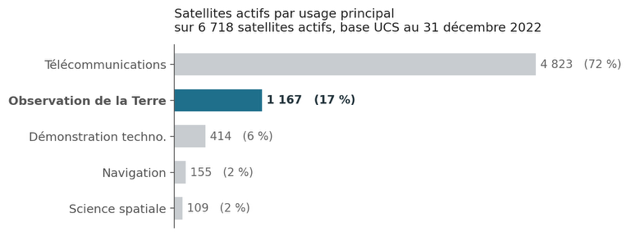
\includegraphics[width=0.85\textwidth]{figures/ot_part_usages.png}
\caption{L'observation de la Terre est le deuxième usage du spatial, loin derrière les télécommunications.}
\end{figure}

Ce ratio de 17\,\% est daté. En août 2026, le décompte de Jonathan McDowell recense \textbf{16\,278 charges utiles actives}, dont 10\,742 Starlink. 
L'effectif d'observation de la Terre, lui, a continué de croître : faute de recensement public à jour, l'ordre de grandeur se situe entre 1\,500 et 2\,000 satellites, mais sa part est retombée autour de 10\,\%.

En prévision, Novaspace attend environ 5\,700 satellites au lancement sur 2025--2034, contre 1\,864 sur la décennie écoulée.

\section{Opérateurs des satellites d'observation}

La concentration est forte : les dix premiers opérateurs détiennent 612 satellites, soit 51\,\% du parc d'observation.

\begin{figure}[!htb]
\centering
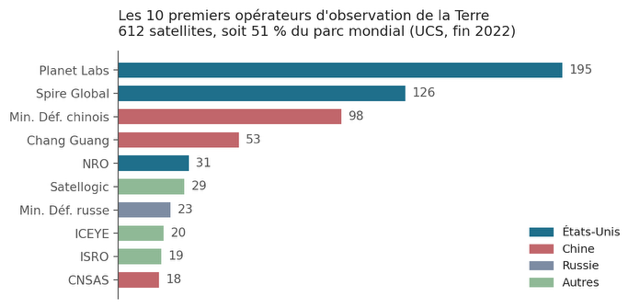
\includegraphics[width=0.85\textwidth]{figures/ot_operateurs.png}
\caption{Trois opérateurs de constellations occupent les trois premières places. Le classement est dominé par les États-Unis et la Chine.}
\end{figure}


\paragraph{ - Nationalités.} À l'intérieur de ce top 10, les opérateurs américains totalisent 352 satellites (Planet, Spire, NRO) et les opérateurs chinois 169 (ministère de la Défense, Chang Guang, Académie des sciences), soit respectivement 30\,\% et 14\,\% du parc mondial. Suivent, très loin derrière, l'Argentine (Satellogic, 29), la Russie (23), la Finlande (ICEYE, 20) et l'Inde (ISRO, 19). L'Europe n'apparaît pas dans ce classement parce que ses satellites sont dispersés entre de nombreux opérateurs nationaux et intergouvernementaux : chacun compte peu d'unités, mais des unités lourdes et très capables.

\paragraph{ - Type d'utilisateur.} Sur les 1\,192 satellites d'observation, 589 servent des clients commerciaux, 327 des clients gouvernementaux civils, 244 des clients militaires et 32 des clients civils divers. 
Le commercial est donc majoritaire, mais il s'agit largement de petits satellites en constellation, alors que pour l'usage militaire et institutionnel ce sont des plateformes uniques et coûteuses.

\paragraph{ - Exemples} 
Le NRO achète massivement de l'imagerie commerciale. 
EUMETSAT est un opérateur civil dont les produits alimentent des chaînes militaires. 
Donc la partition commercial/civil/militaire décrit un mode de financement, mais concretement les satellites concentrent souvent plusieurs usages

\textbf{Landsat-1} (1972) ouvre la brèche civile : imagerie multispectrale, données distribuées à la communauté scientifique. 

\textbf{Meteosat-1} (1977) installe la météorologie géostationnaire européenne. 

\textbf{SPOT-1} (1986) est le premier satellite conçu pour vendre ses images, et le CNES en fait un instrument de politique industrielle. 

\textbf{ERS-1} (1991) apporte le radar imageur européen, insensible aux nuages et à la nuit.

\textbf{IKONOS} (1999), premier satellite privé sous le mètre de résolution, autorisé par une décision américaine de 1994 de libéraliser l'imagerie haute résolution. 

\textbf{Flock-1} (2014, Planet) déploie les premiers CubeSats d'imagerie en constellation

\textbf{Sentinel-1A} (2014) inaugure Copernicus et sa politique de données entièrement libres et gratuites. 

Depuis 2024, le \textbf{Starshield} du NRO (plus de 150 satellites) transpose la logique de constellation pour du renseignement militaire.

\section{Types d'orbites}

\begin{figure}[!htb]
\centering
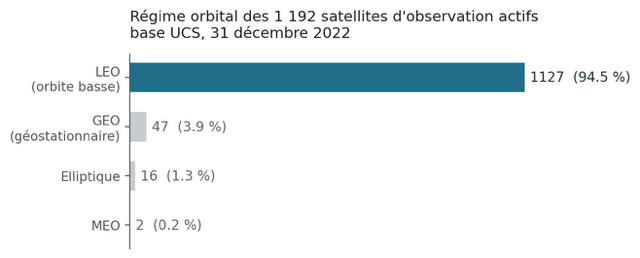
\includegraphics[width=0.80\textwidth]{figures/ot_orbites.png}
\caption{L'observation de la Terre est presque exclusivement LEO.}
\end{figure}


\paragraph{L'orbite héliosynchrone (SSO), 500--900 km} 
C'est l'orbite typique de l'imagerie, optique comme radar. 
Son intérêt : le plan orbital tourne à la même vitesse que la Terre autour du Soleil, si bien que le satellite repasse toujours à la même heure solaire locale. 
L'éclairement est constant d'un passage à l'autre, ce qui rend les images comparables dans le temps, condition indispensable pour détecter un changement plutôt qu'un effet d'ombre.

Cette propriété s'obtient en exploitant l'aplatissement terrestre : 
le terme $J_2$ du potentiel fait dériver le nœud ascendant d'un angle
$$
\dot{\Omega} \;=\; -\frac{3}{2}\,\frac{J_2 R_\oplus^2}{a^2(1-e^2)^2}\, n\cos i,
$$
et il suffit d'égaler cette dérive à la révolution apparente du Soleil ($0{,}9856^\circ$/jour) pour fixer l'inclinaison. 
Donc si on choisit une altitude, l'inclinaison est fixée.

\begin{figure}[!htb]
\centering
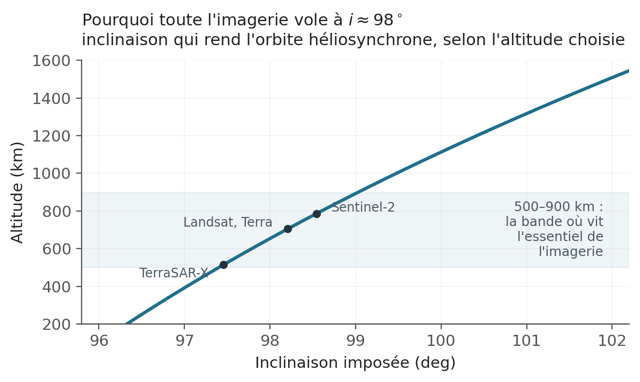
\includegraphics[width=0.78\textwidth]{figures/ot_sso.png}
\caption{Altitude et inclinaison en orbite héliosynchrone}
\end{figure}

\textbf{Les satellites de tous types se retrouvent dans une bande orbitale resserrée.}

\paragraph{L'orbite altimétrique, 1\,336 km à $i = 66^\circ$.} 
Réservée à la mesure de la hauteur des océans (Jason-3, Sentinel-6). 
L'inclinaison de $66^\circ$ n'est pas héliosynchrone : le satellite voit comme ça les marées océaniques à des phases différentes. 
L'altitude élevée réduit par ailleurs la traînée, donc les manœuvres, ce qui préserve la stabilité de la mesure.

\paragraph{L'orbite géostationnaire, 35\,786 km pour la météo.} 
Une quarantaine de satellites seulement, mais ils fournissent l'imagerie en continu d'un hémisphère entier, toutes les dix minutes (Meteosat, GOES, Himawari). 

\paragraph{Les orbites rétrogrades israéliennes, $i \approx 142^\circ$.} 
Un cas particulier purement géographique : Israël lance vers l'ouest, au-dessus de la Méditerranée, pour éviter de survoler ses voisins au décollage. 

\section{Missions des satellites d'observation}

\subsection*{Surveillance des terres et du climat}

\begin{center}
\footnotesize\setlength{\tabcolsep}{4pt}
\begin{tabular}{lllll}
\toprule
Satellite & NORAD & Lancé & Opérateur & Mission \\
\midrule
Terra & 25994 & 1999 & NASA & climat, MODIS/ASTER, SSO 705 km \\
Aqua & 27424 & 2002 & NASA & cycle de l'eau, SSO 705 km \\
Envisat & 27386 & 2002 & ESA & environnement, \textbf{inactif depuis 2012} \\
Landsat-8 & 39084 & 2013 & NASA/USGS & occupation des sols, SSO 705 km \\
Landsat-9 & 49260 & 2021 & NASA/USGS & continuité Landsat depuis 1972 \\
Sentinel-1A / 1C / 1D & 39634 \dots 66315 & 2014--2025 & Copernicus & radar tout-temps, SSO 693 km \\
Sentinel-2A / 2B & 40697 / 42063 & 2015 / 2017 & Copernicus & optique 10 m, agriculture \\
\bottomrule
\end{tabular}
\end{center}

\noindent Exigence : la continuité temporelle de la mesure. 


\subsection*{Météorologie et océanographie}

\begin{center}
\footnotesize\setlength{\tabcolsep}{4pt}
\begin{tabular}{lllll}
\toprule
Satellite & NORAD & Lancé & Opérateur & Mission \\
\midrule
Suomi-NPP & 37849 & 2011 & NASA/NOAA & météo et climat, SSO 824 km \\
NOAA-20 & 43013 & 2017 & NOAA & météo opérationnelle \\
Meteosat-11 & 40732 & 2015 & EUMETSAT & météo GEO \\
MTG-I1 & 54743 & 2022 & EUMETSAT & météo GEO 3\textsuperscript{e} génération \\
GOES-16 & 41866 & 2016 & NOAA & météo GEO, $75{,}2^\circ$\,W \\
Jason-3 & 41240 & 2016 & EUMETSAT/NOAA & niveau des mers, $i = 66^\circ$ \\
Sentinel-6 MF & 46984 & 2020 & UE/US & successeur de Jason \\
Saral & 39086 & 2013 & ISRO/CNES & altimétrie Ka, SSO 800 km \\
CryoSat-2 & 36508 & 2010 & ESA & épaisseur des glaces, $i = 92^\circ$ \\
Sentinel-3A / 3B & 41335 / 43437 & 2016 / 2018 & Copernicus & océan et surfaces continentales \\
\bottomrule
\end{tabular}
\end{center}

\noindent Exigence : la stabilité de la mesure. Un altimètre doit garder son orbite au mètre près pendant des décennies pour que la tendance du niveau marin reste détectable.

\subsection*{Systèmes commerciaux}

\begin{center}
\footnotesize\setlength{\tabcolsep}{4pt}
\begin{tabular}{lllll}
\toprule
Système & NORAD & Lancé & Opérateur & Mission \\
\midrule
GeoEye-1 & 33331 & 2008 & Maxar (US) & optique 0,41 m \\
WorldView-3 & 40115 & 2014 & Maxar (US) & optique 0,31 m, la plus fine du civil \\
Pléiades-1A/1B & 38012 / 39019 & 2011 / 2012 & CNES-Airbus (FR) & optique 0,7 m, \textbf{dual} \\
Pléiades Neo 3/4 & --- & 2021 & Airbus (FR) & optique 0,30 m \\
SPOT-6/7 & 38755 / 40053 & 2012 / 2014 & Airbus (FR) & optique 1,5 m, large fauchée \\
TerraSAR-X & 31698 & 2007 & DLR-Airbus (DE) & radar bande X, SSO 514 km \\
TanDEM-X & 36605 & 2010 & DLR-Airbus (DE) & modèle d'élévation mondial \\
Dove / SkySat & constellation & 2014--- & Planet (US) & revisite quotidienne, 475--500 km \\
ICEYE & constellation & 2018--- & ICEYE (FI) & radar X, surveillance d'inondations \\
Capella & constellation & 2020--- & Capella (US) & radar X à la demande \\
\bottomrule
\end{tabular}
\end{center}

\noindent Exigence : revisite. Voir le même point plusieurs fois par jour, quitte à sacrifier de la résolution. C'est ce qui justifie économiquement la constellation.

\subsection*{Systèmes militaires}

\begin{center}
\footnotesize\setlength{\tabcolsep}{4pt}
\begin{tabular}{lllll}
\toprule
Système & NORAD & Lancé & Pays & Mission \\
\midrule
CSO-1 & 43866 & 2018 & France & reconnaissance, SSO 800 km \\
CSO-2 & 47305 & 2020 & France & identification fine, SSO 480 km \\
CSO-3 & 63156 & 2025 & France & reconnaissance, SSO 800 km \\
USA-224 (KH-11) & 37348 & 2011 & États-Unis & optique, orbite elliptique $270\times986$ km \\
Starshield & multiples & 2024--- & États-Unis & $>$150 satellites, constellation proliférée \\
Yaogan / Gaofen & multiples & 2006--- & Chine & imagerie et écoute, SSO et $i \approx 35$--$63^\circ$ \\
Ofek-16 & --- & 2020 & Israël & optique, orbite rétrograde $i \approx 142^\circ$ \\
COSMO-SkyMed 2G & multiples & 2019--- & Italie & radar X, \textbf{dual} \\
\bottomrule
\end{tabular}
\end{center}

\noindent Remarque : une partie des charges utiles de sécurité nationale américaines n'est pas publiée au catalogue public. 
Leurs éléments orbitaux ne proviennent alors que du réseau d'observateurs indépendant (tel Aldoria !), avec une précision et une cadence forcément inférieures qu'avec les données officielles.

\section{Manœuvres des satellites d'observation}

Deux types d'impulsions classiques.

\begin{itemize}
  \item L'impulsion \textbf{tangentielle} in-plane change l'altitude. Manœuvre d'entretien courante.
  \item L'impulsion \textbf{hors-plan} (perpendiculaire au plan orbital) change l'inclinaison.  Plus rare et plus coûteuse
\end{itemize}


\paragraph{En orbite basse : il faut compenser la traînée.} L'atmosphère résiduelle fait perdre continûment de l'altitude. Le satellite la regagne par une impulsion tangentielle unique, toutes les quelques semaines. S'y ajoutent une à deux manœuvres hors-plan par an pour maintenir l'heure locale du passage.

\paragraph{En orbite géostationnaire : rester sur le même point latitude, longitude} Un satellite géostationnaire doit tenir une fenêtre en longitude, typiquement $\pm 0{,}05^\circ$ à $\pm 0{,}1^\circ$. 
Le champ de gravité terrestre n'étant pas parfaitement symétrique, il dérive lentement vers l'un des deux points d'équilibre ; on le renvoie au départ par une \emph{paire} d'impulsions encadrant le cycle de dérive. Ce maintien Est-Ouest est peu coûteux (quelques m/s par an). L'essentiel du budget passe dans le maintien Nord-Sud, qui contre une dérive d'inclinaison luni-solaire d'environ $0{,}85^\circ$ par an, pour près de 50 m/s annuels.

\paragraph{Cas particuliers} 
Planet maintient le phasage de sa constellation Dove sans jamais pousser, en modulant l'orientation des satellites pour jouer sur leur traînée aérodynamique. 
Et les plateformes à propulsion électrique poussent en continu, à très faible niveau, pendant des heures ou des jours. 
Dans les deux cas il n'y a plus d'impulsions, et ces objets qui deviennent de plus en plus nombreux constituent le cas difficile de toute analyse de trajectoire (mon expérience sur les manoeuvres et les patterns de satellites le confirme...)

\vspace{0.6em}
\noindent\rule{\textwidth}{0.4pt}
\footnotesize
\textbf{Sources.} Effectifs et répartitions par usage, opérateur et orbite : \emph{UCS Satellite Database} , synthèses Pixalytics. Décompte actuel des satellites actifs et bilan 2025 : \emph{Jonathan's Space Report} (planet4589.org), \emph{Space Activities in 2025}. Trafic de lancement : ESA Space Debris Office, \emph{Annual Space Environment Report} 2026. Prévisions de lancement : Novaspace, \emph{Earth Observation Satellite Systems}. Identifiants NORAD et dates de lancement recoupés sur SATCAT.

\end{document}
